%%%%%%%% ICML 2021 EXAMPLE LATEX SUBMISSION FILE %%%%%%%%%%%%%%%%%

\documentclass{article}

% Recommended, but optional, packages for figures and better typesetting:
\usepackage{microtype}
\usepackage{graphicx}
\usepackage{subfigure}
\usepackage{booktabs} % for professional tables

% hyperref makes hyperlinks in the resulting PDF.
% If your build breaks (sometimes temporarily if a hyperlink spans a page)
% please comment out the following usepackage line and replace
% \usepackage{icml2021} with \usepackage[nohyperref]{icml2021} above.
\usepackage{hyperref}

% Attempt to make hyperref and algorithmic work together better:
\newcommand{\theHalgorithm}{\arabic{algorithm}}

% Use the following line for the initial blind version submitted for review:
\usepackage[accepted]{icml2021}

% If accepted, instead use the following line for the camera-ready submission:
%\usepackage[accepted]{icml2021}

% The \icmltitle you define below is probably too long as a header.
% Therefore, a short form for the running title is supplied here:
\icmltitlerunning{Reinforcement Learning 2023 Assignment 2}

\begin{document}

\twocolumn[
\icmltitle{Reinforcement Learning 2023, Master CS, Leiden University \\
   Assignment 2 on Deep Q Learning (DQN)}



% It is OKAY to include author information, even for blind
% submissions: the style file will automatically remove it for you
% unless you've provided the [accepted] option to the icml2021
% package.

% List of affiliations: The first argument should be a (short)
% identifier you will use later to specify author affiliations
% Academic affiliations should list Department, University, City, Region, Country
% Industry affiliations should list Company, City, Region, Country

% You can specify symbols, otherwise they are numbered in order.
% Ideally, you should not use this facility. Affiliations will be numbered
% in order of appearance and this is the preferred way.
\icmlsetsymbol{equal}{*}


\begin{icmlauthorlist}
\icmlauthor{Tom Stein (s3780120)}{lu}
\icmlauthor{Tom Stein (s3780120)}{lu}
\icmlauthor{Tommaso Ancilli (s3674657)}{lu}
\end{icmlauthorlist}
   
\icmlaffiliation{lu}{Faculty of Science, Leiden University, Leiden, The Netherlands}

\icmlcorrespondingauthor{Tom Stein}{tom.stein@tu-dortmund.de}
\icmlcorrespondingauthor{Tommaso Ancilli}{tommaso.ancilli@student.unisi.it}

% You may provide any keywords that you
% find helpful for describing your paper; these are used to populate
% the "keywords" metadata in the PDF but will not be shown in the document
\icmlkeywords{Reinforcement Learning, Machine Learning}

\vskip 0.3in
]

% this must go after the closing bracket ] following \twocolumn[ ...

% This command actually creates the footnote in the first column
% listing the affiliations and the copyright notice.
% The command takes one argument, which is text to display at the start of the footnote.
% The \icmlEqualContribution command is standard text for equal contribution.
% Remove it (just {}) if you do not need this facility.

%\printAffiliationsAndNotice{}  % leave blank if no need to mention equal contribution
\printAffiliationsAndNotice{\icmlEqualContribution} % otherwise use the standard text.

\begin{abstract}
This assignment report focuses on Deep Q Learning (DQN)
with an application to the CartPole environment. 
The basic concept of DQN is introduced along with the experience replay 
and target network improvements.
A hyperparameter scan is used to empirically compare the performance of
the different models and discuss the results.    
A high degree of instability in the training process was observed, 
which is, to some extent, mitigated by specific adjustments of the parameters.
\end{abstract}

\section{Introduction}
\label{sec_introduction}
In this assignment, an agent has to learn how to balance a pole in the vertical position. 
The environment presented is a well known and well defined physical problem, being a reverse pendulum attached to a carriage through a join. 
The goal of this learning task is to keep the pole in place while moving the cart left or right.
The possible action space is made up by a set of only two possible movements ${0,1}$, where $0$: the cart is pushed to the left; $1$: the cart is pushed to the right. 
The state space is composed of four values: position and velocity of the cart, angle and angular velocity of the pendulum.
The agent receives a reward of $+1$ for every action performed that results in keeping the pole in an equilibrium state. 
The environment is reset to the initial condition every time that the value of the angle between the pole and the vertical line is bigger than $15^\circ$ or when the cart leaves the range $(-2,4;2,4)$. 
As it has been coded by OpenAi, the agent has been able to master the game correctly if the total reward is $475$\\.
The old paradigm, where all the q-values could be stored in a table and updated directly to determine the optimal policy, is not suitable anymore. 
The reason lies in the exponential amount of memory required to store all the possible states ( curse of dimensionality). 
Given the impossibility of memorizing all the possible states, the agent has to learn how to generalize to unseen data. 
This can be done through the application of deep learning. It is known that an Artificial Neural Network has the property to approximate any function \cite{Cybenko}, enabling the possibility of inferring an unseen state and having a more compact representation of the solution itself. 
The resulting algorithm, generated by the union of Deep learning and Q-learning, is called Deep Q-Networks algorithm (DQN). 
In this report, the neural network has to approximate the Q-values using a parameterized function. This approach is also called value-based.
\begin{equation}
    Q_{\theta} :  s \rightarrow q
\end{equation}
where, $s \in S$ where $S$ represents the set of all the possible states and $q$ is the Q-values of the admissible actions.\\
In the following chapters, the following points will be addressed. 
In section 2\ref{sec_Methodology}, the underlying theories regarding the separate approaches will be shown.
Section 3\ref{sec_results} is dedicated to the discussion of the optimal configuration for the hyper-parameters tuned on the DQN architecture, which exploits the advantages of replay buffer and target network. 
In this portion of the report the parameters are tweaked individually, which places this unit at the opposite end of the section 5\ref{sec_bonus}. 
Thereupon, this section is dedicated to study the relationship that each hyper-parameter has with the others.
Finally, section 4\ref{sec_discussion} is devoted to give a better insight into what could have been improved.\\
As a baseline comparison to juxtapose to the different solution will be the random one. In this one, the agent performs random moves, and the average cumulative reward is set to $22.4$.

\section{Methodology}
\label{sec_Methodology}

\subsection{DQN}

\subsection{Experience Replay}

\subsection{Target Network}



\section{Results}
\label{sec_results}

\subsection{DQN with ER and TN}

\subsection{DQN ablation study}
% Show what happens if we cut out parts of the model architecture. 

\section{Discussion}
\label{sec_discussion}
% Discuss results in summary here


\section{Hyperparameter Scan - Bonus}
\label{sec_bonus}
In the previous sections, only individual hyperparameters were analyzed in isolation. 
This approach does not take into account the dependencies between the different hyperparameters 
such as learning rate and batch size \cite{DBLP:conf/iclr/SmithKYL18}. 
For this reason, a comprehensive hyperparameter scan was performed, in which models were trained on random combinations of the hyperparameters. 
In the definition of the hyperparameter space \footnote{\texttt{wandb\_sweep\_config.yaml}} 
no continuous value ranges like $[0.8, 1.0]$ were intentionally used but a preselection of discrete values to be able to group and plot the results more easily. 
The space contains about 300 million combinations. 
To search this large space in a reasonable time, several parallel experiments have to be performed. 
For this purpose, the platform Weights and Biases \cite{wandb} was used to log all training runs and to orchestrate the hyperparameter scan across multiple computers. 
The results are shown in \autoref{sec_hyperparameter_scan_results}, 
% TODO Update link to wandb
but can also be viewed interactively online\footnote{\url{https://api.wandb.ai/links/rl-leiden/xttn9bdo}}. 

The results again illustrate the instability caused by wrong parameter selection or catastrophic forgetting, 
since numerous runs only achieve poor results.
% TODO interpret results 
Apart from this, there are also some positive findings, such as .....

% In the unusual situation where you want a paper to appear in the
% references without citing it in the main text, use \nocite
\nocite{DBLP:books/sp/Plaat22}

\bibliography{main}
\bibliographystyle{icml2021}


\appendix
\section{Hyperparameter Scan Results}
\label{sec_hyperparameter_scan_results}

% TODO Update image
\begin{figure*}[h!]
   \centering
   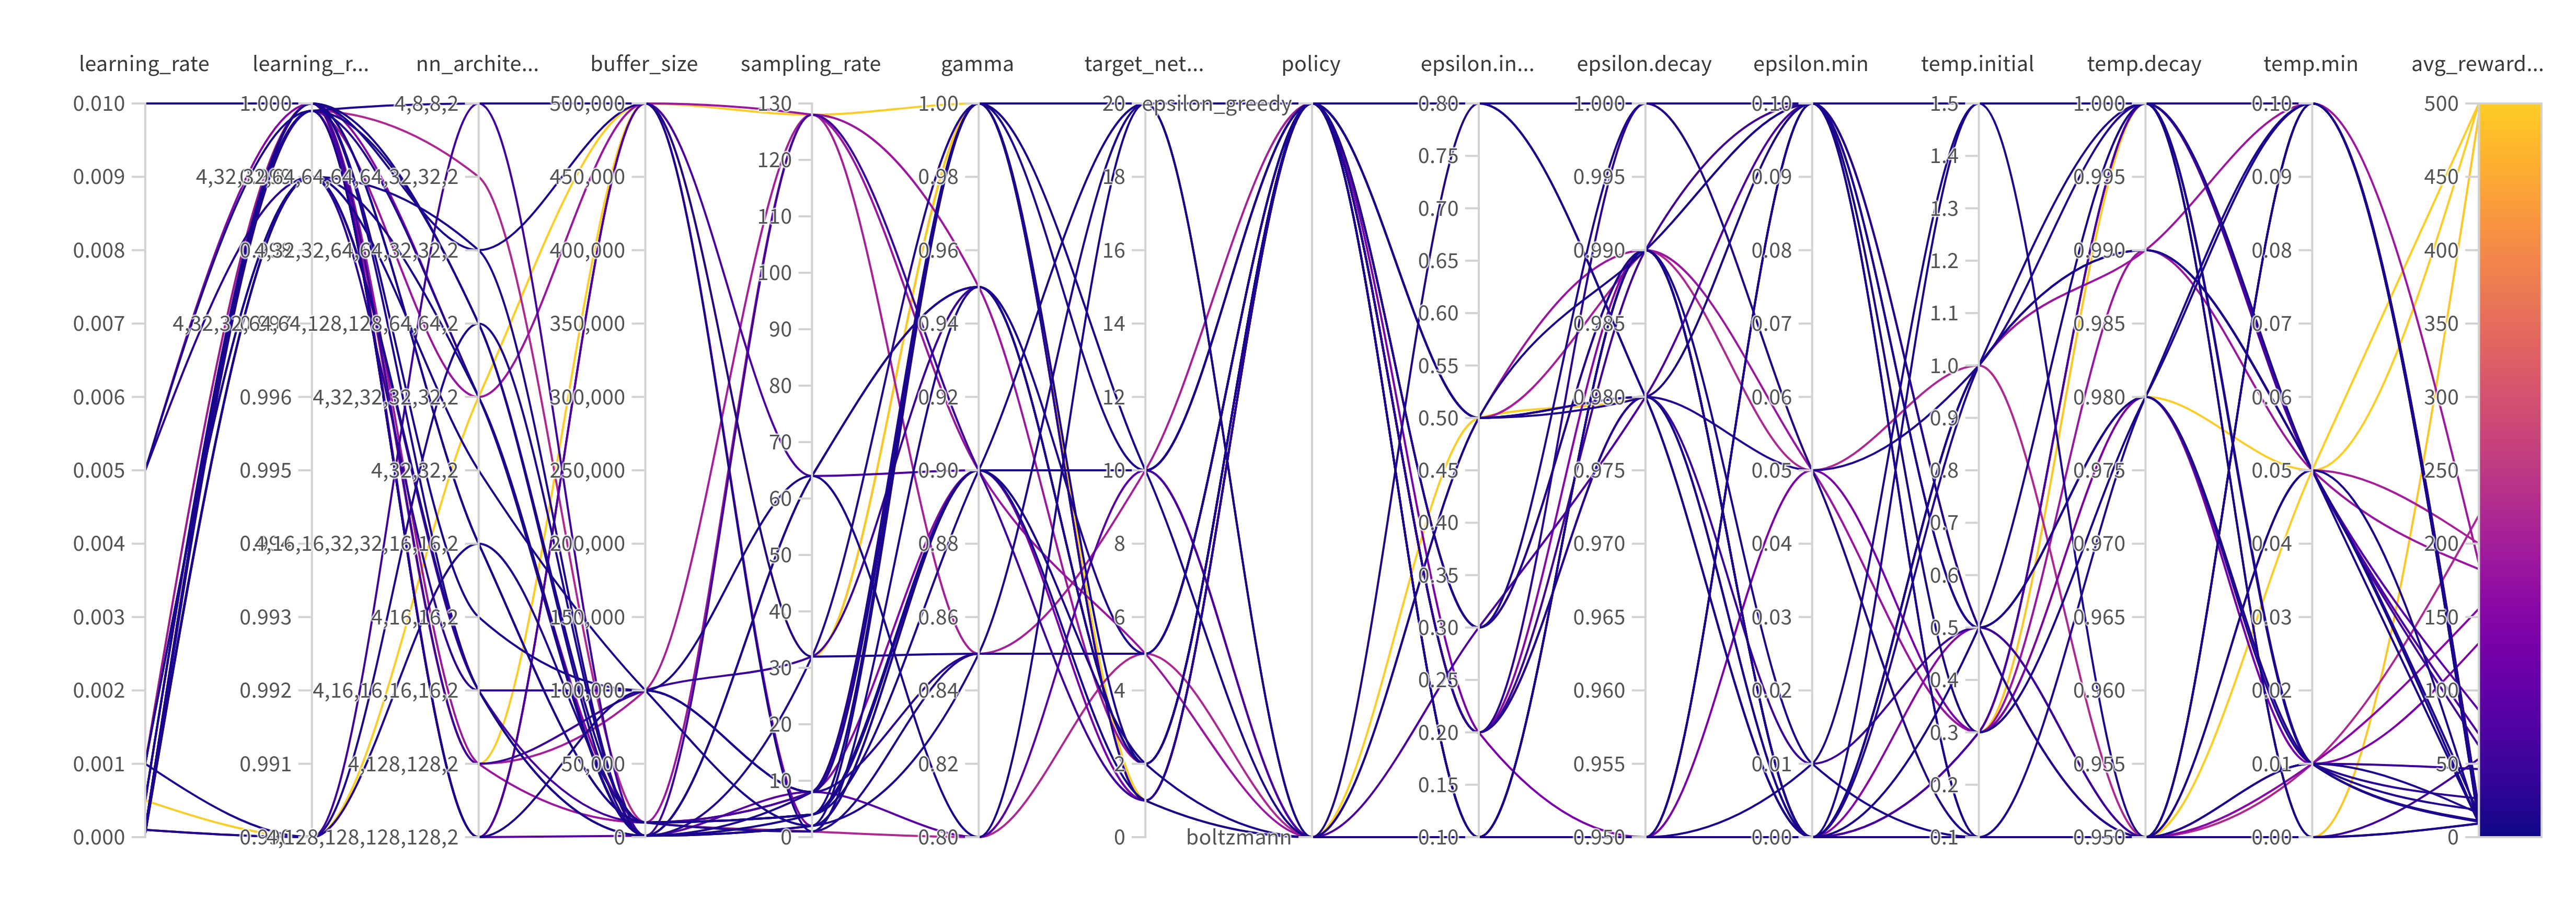
\includegraphics[width=\textwidth]{assets/hyperparamter-scan/W&B Chart 3_30_2023, 2 24 25 PM.png}
   \caption{Parallel axis plot of the hyperparameter scan. 
      Each line shows a single parameter configuration that was evaluated. 
      The color indicates the performance measured by the average of the last 100 epochs (see legend on the right). 
      Higher average reward (yellow) is better.
   }
   \label{fig_hyperparameter_scan_parallel_axis}
\end{figure*}


\end{document}


% This document was modified from the file originally made available by
% Pat Langley and Andrea Danyluk for ICML-2K. This version was created
% by Iain Murray in 2018, and modified by Alexandre Bouchard in
% 2019 and 2021. Previous contributors include Dan Roy, Lise Getoor and Tobias
% Scheffer, which was slightly modified from the 2010 version by
% Thorsten Joachims & Johannes Fuernkranz, slightly modified from the
% 2009 version by Kiri Wagstaff and Sam Roweis's 2008 version, which is
% slightly modified from Prasad Tadepalli's 2007 version which is a
% lightly changed version of the previous year's version by Andrew
% Moore, which was in turn edited from those of Kristian Kersting and
% Codrina Lauth. Alex Smola contributed to the algorithmic style files.
